% !TEX TS-program = pdflatex
% !TEX encoding = UTF-8 Unicode

% This is a simple template for a LaTeX document using the "article" class.
% See "book", "report", "letter" for other types of document.

\documentclass[11pt]{article} % use larger type; default would be 10pt

\usepackage[utf8]{inputenc} % set input encoding (not needed with XeLaTeX)

%%% Examples of Article customizations
% These packages are optional, depending whether you want the features they provide.
% See the LaTeX Companion or other references for full information.

%%% PAGE DIMENSIONS
\usepackage{geometry} % to change the page dimensions
\geometry{a4paper} % or letterpaper (US) or a5paper or....
% \geometry{margin=2in} % for example, change the margins to 2 inches all round
% \geometry{landscape} % set up the page for landscape
%   read geometry.pdf for detailed page layout information

\usepackage{graphicx} % support the \includegraphics command and options

% \usepackage[parfill]{parskip} % Activate to begin paragraphs with an empty line rather than an indent

%%% PACKAGES
\usepackage{booktabs} % for much better looking tables
\usepackage{array} % for better arrays (eg matrices) in maths
\usepackage{paralist} % very flexible & customisable lists (eg. enumerate/itemize, etc.)
\usepackage{verbatim} % adds environment for commenting out blocks of text & for better verbatim
\usepackage{subfig} % make it possible to include more than one captioned figure/table in a single float
% These packages are all incorporated in the memoir class to one degree or another...

%%% HEADERS & FOOTERS
\usepackage{fancyhdr} % This should be set AFTER setting up the page geometry
\pagestyle{fancy} % options: empty , plain , fancy
\renewcommand{\headrulewidth}{0pt} % customise the layout...
\lhead{}\chead{}\rhead{}
\lfoot{}\cfoot{\thepage}\rfoot{}

%%% SECTION TITLE APPEARANCE
\usepackage{sectsty}
\allsectionsfont{\sffamily\mdseries\upshape} % (See the fntguide.pdf for font help)
% (This matches ConTeXt defaults)

%%% ToC (table of contents) APPEARANCE
\usepackage[nottoc,notlof,notlot]{tocbibind} % Put the bibliography in the ToC
\usepackage[titles,subfigure]{tocloft} % Alter the style of the Table of Contents
\renewcommand{\cftsecfont}{\rmfamily\mdseries\upshape}
\renewcommand{\cftsecpagefont}{\rmfamily\mdseries\upshape} % No bold!

%%% END Article customizations

%%% The "real" document content comes below...

\title{Brief Article}
\author{The Author}
%\date{} % Activate to display a given date or no date (if empty),
         % otherwise the current date is printed 

\begin{document}


\section{Linear Regression Analysis}

\subsection{Introduction}
Linear regression is used when you want to predict the value of a variable based on the value of another variable. The variable we want to predict is called the dependent variable (or sometimes, the outcome variable). The variable we are using to predict the other variable's value is called the independent variable (or sometimes, the predictor variable).


For example, you could use linear regression to understand whether exam performance can be predicted based on revision time; whether cigarette consumptions can be predicted based on smoking duration; and so forth. If you have two or more independent variables, rather than just one, you need to use \textbf{\textit{multiple regression}}.

SPSS can be used to carry out linear regression, as well as interpret and report the results from this test. However, before we introduce you to this procedure, you need to understand the different assumptions that your data must meet in order for linear regression to give you a valid result. We discuss these assumptions next.


\subsection{Assumptions}
When you choose to analyse your data using linear regression, part of the process involves checking to make sure that the data you want to analyse can actually be analysed using linear regression. You need to do this because it is only appropriate to use linear regression if your data is appropriate for six assumptions that are required for linear regression to give you a valid result.

In practice, checking for these six assumptions just adds a little bit more time to your analysis, requiring you to click a few more buttons in SPSS when performing your analysis, as well as think a little bit more about your data, but it is not a difficult task.

Often when analysing your own data using SPSS, one or more of these assumptions is violated (i.e., not met). This is not uncommon when working with real-world data rather than textbook examples, which often only show you how to carry out linear regression when everything goes well. However, even when your data fails certain assumptions, there is often a solution to overcome this. First, let’s take a look at these six assumptions:

\begin{itemize}
\item \textbf{Assumption 1}: Your two variables should be measured at the interval or ratio level (i.e., they are continuous). Examples of variables that meet this criterion include revision time (measured in hours), intelligence (measured using IQ score), exam performance (measured from 0 to 100), weight (measured in kg), and so forth. You can learn more about interval and ratio variables in our article: Types of Variable.

\item \textbf{Assumption 2}: There needs to be a linear relationship between the two variables. Whilst there are a number of ways to check whether a linear relationship exists between your two variables, we suggest creating a scatter-plot using SPSS, where you can plot the dependent variable against your independent variable, and then visually inspect the scatter-plot to check for linearity. Your scatter-plot may look something like one of the following:

If the relationship displayed in your scatterplot is not linear, you will have to either run a non-linear regression analysis or \textbf{\textit{transform}} your data, which you can do using SPSS.

 It is important to learn how to:
\begin{itemize} 
\item[(a)] create a scatterplot to check for linearity when carrying out linear regression using SPSS; 
\item[(b)] interpret different scatterplot results; and \item[(c)] transform your data using SPSS if there is not a linear relationship between your two variables.
\end{itemize}

\begin{figure}[h!]
\begin{centering}
  % Requires \usepackage{graphicx}
  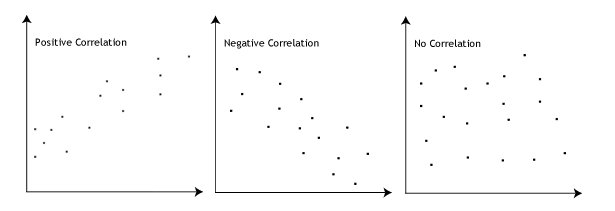
\includegraphics[width=10cm]{Regre1.jpg}\\
  \caption{Types of Linear Relationship}
\end{centering}
\end{figure}

\item \textbf{Assumption 3}: There should be no significant outliers.\\ Outliers are simply single data points within your data that do not follow the usual pattern (e.g., in a study of 100 students’ IQ scores, where the mean score was 108 with only a small variation between students, one student had a score of 156, which is very unusual, and may even put her in the top 1\% of IQ scores globally). The following scatterplots highlight the potential impact of outliers:

The problem with outliers is that they can have a negative effect on the regression equation that is used to predict the value of the dependent (outcome) variable based on the independent (predictor) variable. This will change the output that SPSS produces and reduce the predictive accuracy of your results. Fortunately, when using SPSS to run linear regression on your data, you can easily include criteria to help you detect possible outliers.
\begin{figure}[h!]
\begin{centering}
  % Requires \usepackage{graphicx}
  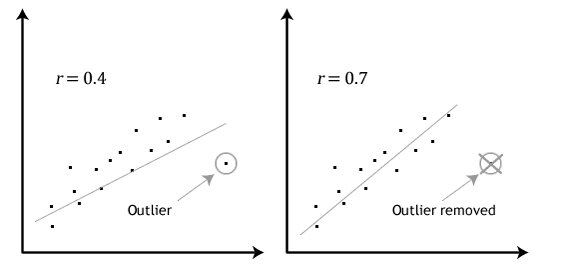
\includegraphics[width=10cm]{Regre2.jpg}\\
  \caption{Effect of an Outlier}
\end{centering}
\end{figure}
%In our enhanced linear regression guide, we: (a) show you how to detect outliers using \textbf{case-wise diagnostics}, which is a simple process when using SPSS; and (b) discuss some of the options you have in order to deal with outliers.
\item \textbf{Assumption 4}: You should have independence of observations, which you can easily check using the Durbin-Watson statistic, which is a simple test to run using SPSS. We explain how to interpret the result of the Durbin-Watson statistic later.

\item \textbf{Assumption 5}:Your data needs to show \textbf{\textit{homoscedasticity}}, which is where the variances along the line of best fit remain similar as you move along the line. 

Whilst we explain more about what this means and how to assess the homoscedasticity of your data in the linear regression line, take a look at the two scatter-plots below, which provide two simple examples: one of data that meets this assumption and one that fails the assumption:

\begin{figure}[h!]
\begin{centering}
  % Requires \usepackage{graphicx}
  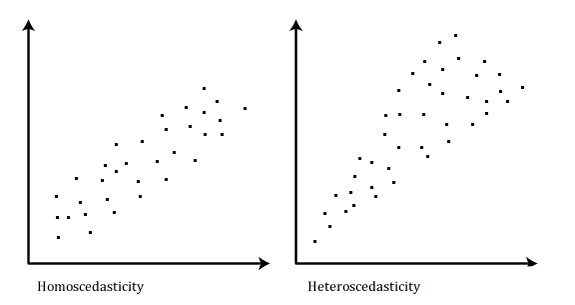
\includegraphics[width=10cm]{Regre3.jpg}\\
  \caption{Constant Variance}
\end{centering}
\end{figure}
When you analyse your own data, you will be lucky if your scatterplot looks like either of the two above. Whilst these help to illustrate the differences in data that meets or violates the assumption of homoscedasticity, real-world data is often a lot more messy. 

%Therefore, in our enhanced linear regression guide, we explain: (a) some of the things you will need to consider when interpreting your data; and (b) possible ways to continue with your analysis if your data fails to meet this assumption.
\item \textbf{Assumption 6}:Finally, you need to check that the residuals (errors) of your two variables are approximately normally distributed (we explain these terms in our enhanced linear regression guide). Two common methods to check this assumption include using either a histogram (with a superimposed normal curve) or by using a Normal P-P Plot.
  %  Again, in our enhanced linear regression guide, we: (a) show you how to check this assumption using SPSS, whether you use a histogram (with superimposed normal curve) or Normal P-P Plot; (b) explain how to interpret these diagrams; and (c) provide a possible solution if your data fails to meet this assumption.

\end{itemize}
You can check assumptions all assumptions except no.1 using SPSS. 

It is recommended to test these assumptions in this order because it represents an order where, if a violation to the assumption is not correctable, you will no longer be able to use a single linear regression (although you may be able to run another statistical test on your data instead). 

Just remember that if you do not run the statistical tests on these assumptions correctly, the results you get when running a linear regression might not be valid.

\subsection{Types of multicollinearity}
%http://online.stat.psu.edu/online/development/stat501/12multicollinearity/02multico_whatis.html

%------------------------------------------------------------------------------------------------------%

There are two types of multicollinearity: 
\begin{itemize}
\item Structural multicollinearity
\item Data-based multicollinearity
\end{itemize}
Structural multicollinearity is a mathematical artifact caused by creating new predictors from other predictors — such as, creating the predictor x2 from the predictor x. 
Data-based multicollinearity, on the other hand, is a result of a poorly designed experiment, reliance on purely observational data, or the inability to manipulate the system on which the data are collected. 
In the case of structural multicollinearity, the multicollinearity is induced by what you have done. Data-based multicollinearity is the more troublesome of the two types of multicollinearity. Unfortunately it is the type we encounter most often!

%------------------------------------------------------------------------------------------------------%

\newpage
 

%------------------------------------------------------------------------------------------------------%

\subsection{Tolerance}
A tolerance close to 1 means there is little multicollinearity, whereas a value close to 0 suggests that multicollinearity may be a threat. The reciprocal of the tolerance is known as the Variance Inflation Factor (VIF). The VIF shows us how much the variance of the coefficient estimate is being inflated by multicollinearity. For example, if the VIF for a variable were 9, its standard error would be three times as large as it would be if its VIF was 1. In such a case, the coefficient would have to be 3 times as large to be statistically significant.

\[ \mbox{Tolerance} = \frac{1}{VIF}\]

\subsection{Variance Inflation Factor}

% http://online.stat.psu.edu/online/development/stat501/12multicollinearity/05multico_vif.html


We learned previously that the standard errors, and hence the variances, of 
the estimated coefficients are inflated when multicollinearity exists. 
So, the variance inflation factor for the estimated coefficient $b_k$, denoted $VIF_k$, 
is just the factor by which the variance is inflated. 

Variance inflation factors k greater than 4 suggest that the multicollinearity should be investigated. 
Variance inflation factors greater than 10 are taken as an indication that the multicollinearity may be unduly influencing the least squares estimates.


%------------------------------------------------------------------------------------------------------%
\section{Missing Data}
%----------------------------------------------------%
\subsection{Types of Missing Data}
\begin{itemize}
\item Missing at Random (MAR)
\item Missing Completely at Random (MCAR)
\item Missing Not at Random (MNAR)
\end{itemize}

%----------------------------------------------------%
\subsection{Traditional Approaches to Missing Data}
\begin{itemize}
\item Listwise Deletion
\item Casewise Deletion
\item Pairwise Deletion
\end{itemize}

In listwise deletion a case is dropped from an analysis because it has a missing value in at least one of the specified variables. The analysis is only run on cases which have a complete set of data.


Pairwise deletion occurs when the statistical procedure uses cases that 
contain some missing data. The procedure cannot include a particular variable 
when it has a missing value, but it can still use the case when analyzing other 
variables with non-missing values. 
A case may contain 3 variables: VAR1, VAR2, and VAR3. 
A case may have a missing value for VAR1, but this does not prevent some statistical 
procedures from using the same case to analyze variables VAR2 and VAR3. Pairwise deletion allows you to use more of your data. However, each computed statistic may be based
on a different subset of cases. This can be problematic. 
For example, a correlation matrix computed using pairwise deletion may not be 
positive semidefinite. That is, it may have negative eigenvalues, which can create problems for various statistical analyses. This can occur because when correlations are computed using different cases, the resulting patterns can be ones that are impossible to produce with complete data.

Note that the means and standard deviations computed when pairwise deletion 
is specified are based on all available data for each variable. 
Correlations are based on all data available for each pair of variables.

The choice between pairwise and listwise deletion of records is limited. The choice between these two types of deletion is not relevant when only one variable is being analyzed. In other situations, missing values may be treated as a valid category. If a record has a missing value for a crucial dependent variable, it probably cannot be used in the analysis. Pairwise vs. listwise is a different choice from the decision on whether to include or exclude user-defined missing values within a procedure. 


%----------------------------------------------------%
http://www-01.ibm.com/support/docview.wss?uid=swg21475199

For example, each missing value can
be imputed from the variable mean of the complete cases,
or it can be imputed from the mean conditional on observed
values of other variables. This approach treats missing values
as if they were known in the complete-data analyses.
Single imputation does not reflect the uncertainty about the
predictions of the unknown missing values, and the resulting
estimated variances of the parameter estimates will be
biased toward zero.

%----------------------------------------------------%
\subsection{Multiple Imputation}
% http://www.ats.ucla.edu/stat/sas/library/multipleimputation.pdf

Multiple imputation provides a useful strategy for dealing
with data sets with missing values. Instead of filling in a
single value for each missing value, the multiple
imputation procedure replaces each missing value with a
set of plausible values that represent the uncertainty about
the right value to impute. These multiply imputed data sets
are then analyzed by using standard procedures for complete
data and then combining the results from all of these analyses.
No matter which complete-data analysis is used, the process
of combining results from different imputed data sets
is essentially the same. This results in valid statistical inferences
that properly reflect the uncertainty due to missing
values.

%----------------------------------------------------%
\subsubsection{Phases of Multiple Imputation}
Multiple imputation inference involves three distinct phases:
\begin{itemize}
\item The missing data are filled in m times to generate m
complete data sets.
\item The m complete data sets are analyzed by using
standard procedures.
\item The results from the m complete data sets are combined
for the inference.
\end{itemize}
%---------------------------------------------------%
\end{document}
%------------------------------------------------------------------------------%\end{document}


